\documentclass[a4paper,10pt]{report}
\usepackage{geometry}\geometry{a4paper,top=3.5cm,bottom=3.5cm,%
left=2.5cm,right=2.5cm,heightrounded,bindingoffset=0mm}
\usepackage[T1]{fontenc}
\usepackage[utf8]{inputenc}
\usepackage[italian]{babel}
\usepackage{graphicx}
\usepackage[export]{adjustbox}%Per il Frame attrono le immagini e il valign
\usepackage{subfig}
\usepackage{amsmath,amsfonts,amssymb,braket,mathrsfs}
\usepackage{float}
\usepackage{tabularx,booktabs}
\usepackage{hyperref}
\usepackage{epsfig}
\usepackage{pdfpages} %Per gli allegati
%\usepackage{minipage}
\usepackage[output-decimal-marker={,}]{siunitx}
\usepackage{tikz}
\usepackage{pgfplots,pgfplotstable}
%\pgfplotsset{compat=1.15} %indica la versione da utilizzare per pgfplot
\usetikzlibrary{patterns} % per il tratteggio
\usepgfplotslibrary{groupplots}
\pgfplotsset{compat=newest}
%\usepackage{stanli}
\usepackage{xspace}% per lo spazio intelligente
\newcommand{\e}{\`E\xspace}  %E'
\usepackage{titlesec} % per formato custom dei titoli dei capitoli
%\usepackage{sideways}%%%
% redefinizione del formato del titolo del capitolo
      % da formato
      %   Capitolo X
      %   Titolo capitolo
      %   a formato
      %      Titolo capitolo 
	\titleformat{\chapter}
        {\normalfont\Huge\bfseries}{}{0em}{}
	\titlespacing*{\chapter}{0pt}{0in}{0.02in}
	\titlespacing*{\section}{0pt}{0.2in}{0.02in}
	\titlespacing*{\subsection}{0pt}{0.10in}{0.02in}
%serve per la didascalia di tabelle e figure:
\usepackage{caption}
\captionsetup{tableposition=top,figureposition=bottom,font=small}\captionsetup{format=hang,labelfont={bf,color=pantone186}} %didascalie a più righe allineate e il nome in grassetto
%non viene allineato a sinistra se la didascalia è corta una sola riga. PERCHé??
\usepackage{xcolor}
%serve per mettere il codice con lo sfondo grigio chiaro
\definecolor{pantone186}{RGB}{206, 17, 38} %il colore del logo UNITN
\definecolor{myGray}{gray}{0.5} %più basso più scuro è
\usepackage{listings} 
\lstset{basicstyle=\scriptsize\ttfamily,
backgroundcolor=\color{lightgray},%
boxpos=c,%
stringstyle=\itshape,		
lineskip=3pt,%
numbers=left,
numberstyle=\tiny,}
\usepackage{lscape}
\usepackage{multirow}
\usepackage{import}
%\usepackage{pythontex}
\begin{document}
%!TEX root = ../TesiTriennaleMeoliNicola.tex
\pagestyle{plain}
\thispagestyle{empty}
\begin{center}
  \begin{figure}[H]
    \centerline{
\psfig{file=IMG/logo_unitn_black_centerNEW.eps,
                        width=0.8\textwidth,trim = 0 0.9cm 0 0.5cm}}
  \end{figure}
\textcolor{pantone186}{\noindent\rule{\textwidth}{.5pt}}

  \Large\textsc{Dipartimento di Ingegneria Civile, Ambientale e Meccanica\\}
  \Large{Corso di Laurea in Ingegneria Civile
  }

  \vspace{3.7 cm} 
  %\Large\textsc{Elaborato finale\\} 
  %\vspace{1 cm} 
  \Huge\textsc{Confronto energetico tra diverse soluzioni edilizie\\}
  
  \vspace{0.2 cm}
  \Large{\it{Analisi termo igrometrica di alcuni pacchetti strutturali composti da differenti materiali. }}


  \vspace{4 cm} 
  \begin{tabular*}{\textwidth}{ l @{\extracolsep{\fill}} r }
  \Large\textsc{Docenti} & \Large\textsc{Studente}\\
  \Large{Rossano Albatici}& \Large{Nicola Meoli 186100}\\
  
  	
  	
  \end{tabular*}

  \vspace{3.1cm} 
  \textcolor{pantone186}{\noindent\rule{\textwidth}{1pt}}
    
  \Large{Anno accademico 2020/21}
  
\end{center}


\tableofcontents
%\setcounter{page}{1}
%Tabelle e figure sulla stessa pagina:
%Le aggiunge all'indice. phantomsection serve per non far casini con hyperref
\clearpage
\begingroup
   %\let\cleardoublepage\relax  % book
    \let\clearpage\relax        % report
        \listoftables
        \phantomsection
        \addcontentsline{toc}{chapter}{Elenco delle tabelle}
        %
        \listoffigures
        \phantomsection
        \addcontentsline{toc}{chapter}{Elenco delle figure}
\endgroup
%

\chapter{nome capitlo 1}
\begin{figure}[htbp]
    \centering
    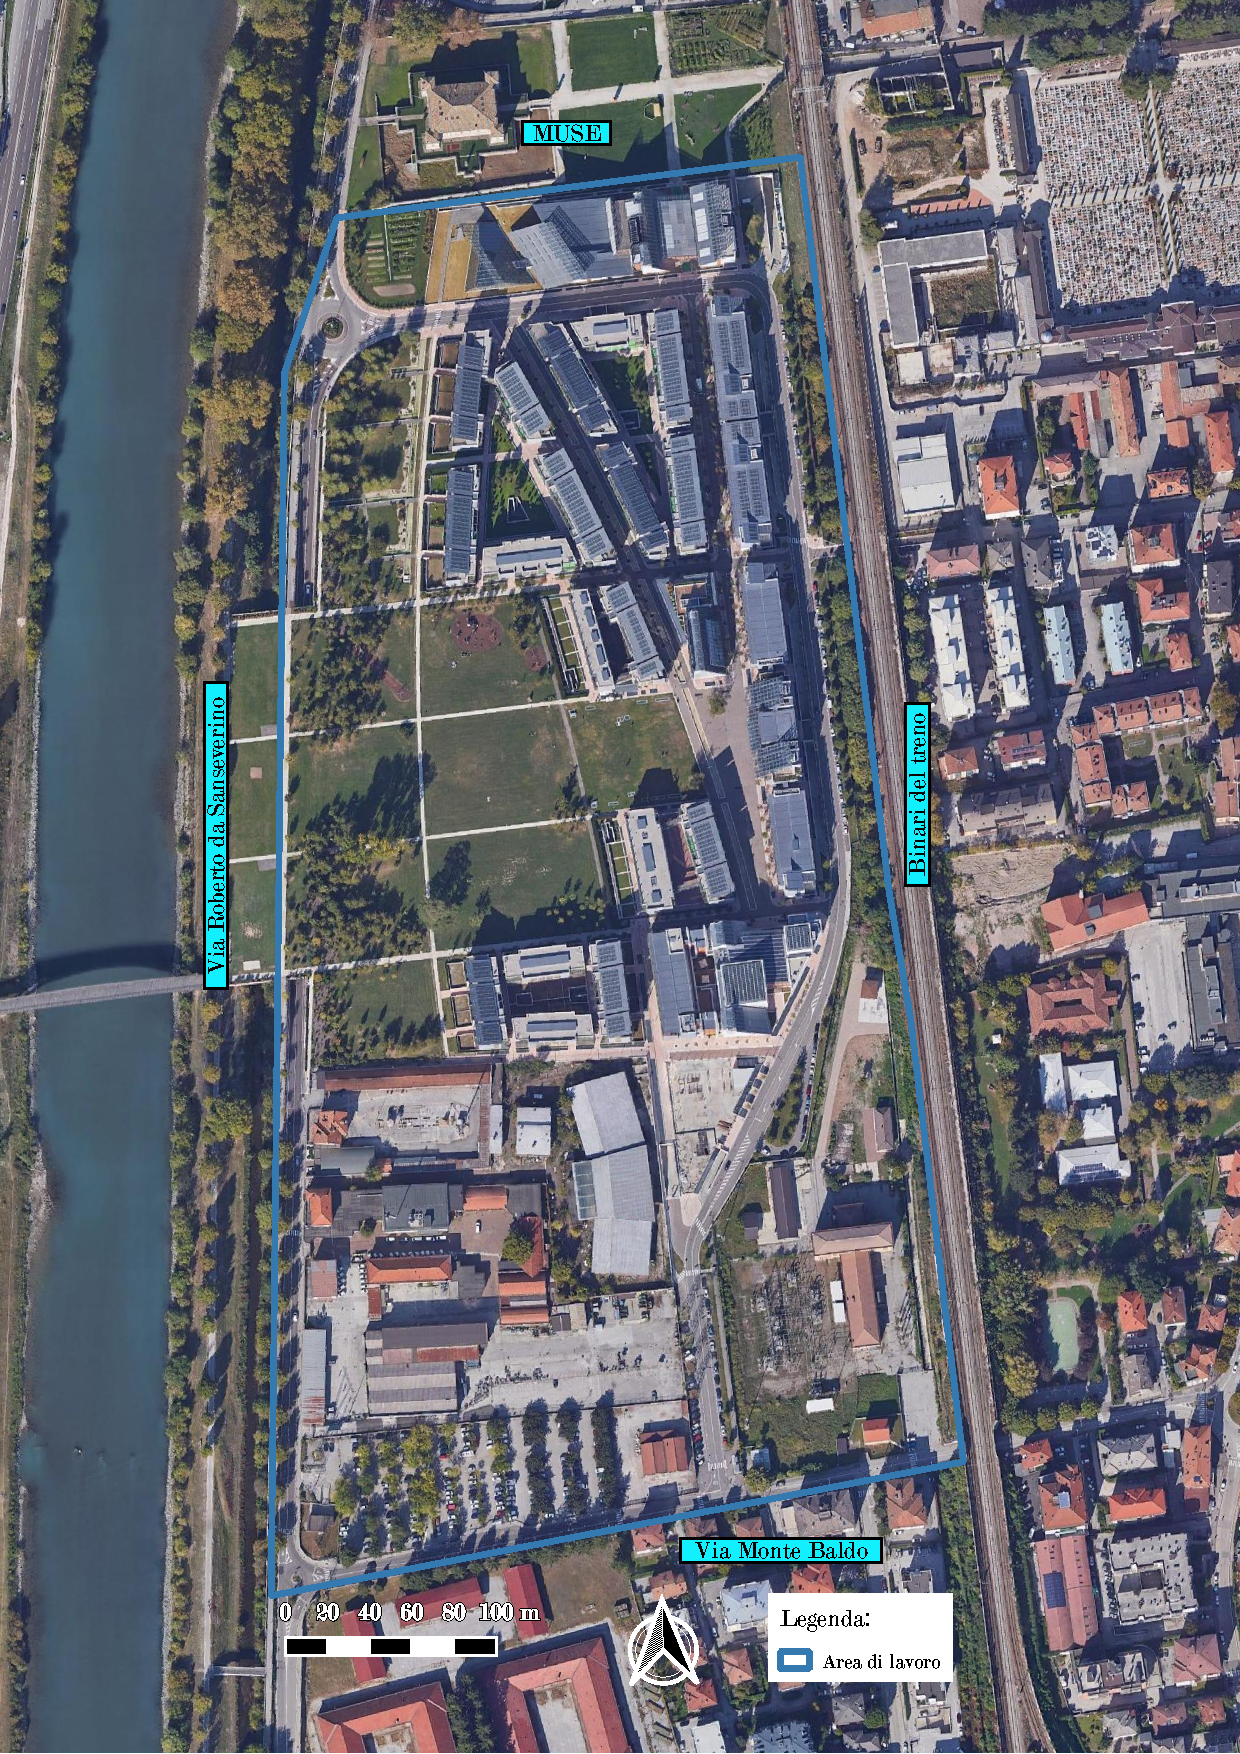
\includegraphics[trim=0cm 0cm 0cm 0cm,clip,frame,width=\textwidth]{IMG/inquadramento.pdf} 
    \caption{Inquadramento dell'area di lavoro}
    \label{fig:inquadramento}
    \end{figure}

\begin{equation}
    i = a \, t_p ^{n - 1}
\end{equation}
\begin{equation}
    CN = \frac{25400}{254 + S}
\end{equation}

\begin{equation}
    T_{\text{dry}} = \frac{3.125}{\sqrt{K_s}}
\end{equation}
Dove $T_{\text{dry}}$ sono i giorni che impiega il suolo completamente saturo a tornare secco e $K_s$ è la conduttività idraulica espressa in \si{inch\per\hour}.
\begin{equation}
    i_m = \frac{h(t_\text{fin}) - h(t_\text{in})}{\Delta t}
\end{equation}
\begin{equation}   
    h(t) = 
    \begin{cases}
        r \, a \left[ \left( \frac{t_p}{r}\right)^n - \left( \frac{t_p - t}{r}\right)^n  \right] & \text{se $t < t_p$}\\
        a \left[ r \left( \frac{t_p}{r}\right)^n + (1-r)\left( \frac{t_p - t}{1 - r}\right)^n  \right] & \text{se $t > t_p$}\\
    \end{cases}
\end{equation}
 


















\begin{landscape}
    \begin{figure}[htb]
        \centering
        \begin{tikzpicture}
            \begin{axis}[
                restrict x to domain=-0:1.5,
                height=15cm,
                width=21cm,
                grid=major,
                xlabel=Tempo trascorso dall'inizio della precipitazione \si{[\hour]},
                ylabel=Deflusso  \si{[\litre\per\second]},
                xtick = {0.5,1,1.5,2,2.5,3,3.5,4},
                %title= ,
                /pgf/number format/.cd,
                use comma,
                1000 sep={\,}
            ]
            \addplot +[mark=none,style=solid,color=red] table[x index=0,y index=1,header=false] {IMG/Total-Inflow/total_inflow_1min.txt};
            \addplot +[mark=none,style=solid,color=green!60!black] table[x index=0,y index=1,header=false] {IMG/Total-Inflow/total_inflow_2min.txt};
            \addplot +[mark=none,style=solid,color=magenta] table[x index=0,y index=1,header=false] {IMG/Total-Inflow/total_inflow_5min.txt};
            \addplot +[mark=none,style=solid,color=cyan] table[x index=0,y index=1,header=false] {IMG/Total-Inflow/total_inflow_10min.txt};
            \addplot +[mark=none,style=solid,color=orange] table[x index=0,y index=1,header=false] {IMG/Total-Inflow/total_inflow_15min.txt};
            \addplot +[mark=none,style=solid,color=teal] table[x index=0,y index=1,header=false] {IMG/Total-Inflow/total_inflow_30min.txt};
            \addplot +[mark=none,style=solid,color=violet] table[x index=0,y index=1,header=false] {IMG/Total-Inflow/total_inflow_45min.txt};
            \legend{1 min,2 min,5 min,10 min,15 min,30 min,45 min}    
            \end{axis}
        \end{tikzpicture}
        \caption{Deflusso del bacino}
        \label{fig:Ietogrammi}
    \end{figure}
\end{landscape}

\begin{landscape}
    \begin{figure}[htb]
        \centering
        \begin{tikzpicture}
            \begin{axis}[
                restrict x to domain=-0:4,
                height=15cm,
                width=21cm,
                grid=major,
                xlabel=Tempo trascorso dall'inizio della precipitazione \si{[\hour]},
                ylabel=Total Inflow  \si{[\litre\per\second]},
                xtick = {0.5,1,1.5,2,2.5,3,3.5,4},
                %title= ,
                /pgf/number format/.cd,
                use comma,
                1000 sep={\,}
            ]
            \addplot +[mark=none,style=solid,color=red] table[x index=0,y index=1,header=false] {IMG/Total-Inflow/total_inflow_5min_Chicago_25anni.txt};
            \end{axis}
        \end{tikzpicture}
        \caption{Andamento dello sforzo assiale agente sul pilastro P27 in funzione dell'altezza}
        \label{fig:IetogrammaFinale}
    \end{figure}   
\end{landscape}
%\chapter{vasche belle  belle}
Al progetto della rete di drenaggio vengono ora aggiunte tre vasche di laminazione in corrispondenza dei tre sbocchi della rete e chiamate rispettivamente: \emph{Nord}, \emph{Centro} e \emph{Sud}.
Lo scopo di tali vasche è quello di fungere da ammortizzatore idraulico venendo dimensionate in modo da contenere la portata massima scaricata nel corpo idrico recettore.

Il predimensionamento delle vasche si articola in un metodo iterativo per far sì di avere il maggior riempimento di esse (prossimo al \SI{100}{\percent}) e parallelamente un \emph{Maximum Outflow} minore della massima portata da mantenere come da progetto. 
Tale portata è calcolata tenendo conte delle prescrizioni legislative per il coefficiente udometrico, che per Trento è pari a $C_{udo} = \SI{20}{\litre\per\second\per\hectare}$, fissando così la portata massima in uscita da scaricare. 

La portata massima da mantenere pertanto diviene:
\begin{equation}
    Q_{max} = C_{udo} \cdot A_{\text{sottobacino}}
    \label{eq:qmax} \quad ,
\end{equation}
dove con $A_{\text{sottobacino}}$ si intende l'area di pertinenza di ciascuna vasca, ovvero la somma delle aree dei sottobacini confluenti in essa.

I parametri da variare nell'iterazione (in fase non esecutiva del progetto) sono l'area della vasca e il diametro dell'orifizio della stessa (o analogamente l'area dell'orifizio -- essendo di sezione cilindrica). 


Come prima iterazione l'area dell'orifizio è calcolata invertendo la formula della forometria della portata uscente e ponendola uguale alla $Q_{max}$:
\begin{equation}
    Q  = C_{eff} A_{\text{orifizio}} \sqrt{2 g h} \overset{!}{=} Q_{max} \quad .
\end{equation}
Si è scelto un coefficiente di efflusso $C_{eff} = \SI{0.65}{}$, avendo una bocca a battente a luce fissa e verticale. 
Mentre l'area della vasca è calcolata dividendo il volume totale da invasare per la profondità della vasca di progetto $h = \SI{1.50}{\metre}$.

Il volume totale da invasare è stato calcolato come sommatoria dell'area compresa tra le due curve (visibili in figura \ref{fig:vasche}) corrispondenti al deflusso nella condotta senza vasca e al deflusso attenuato dalla presenza della vasca. 
Le funzioni delle curve sono state discretizzate con un intervallo di 60 secondi e la parte compresa tra loro è stata calcolata come differenza delle due aree sottese e ottenute tramite il metodo dei trapezi.
\begin{figure}[p]
    \centering
    \begin{tikzpicture}
        \begin{axis}[
            %restrict x to domain=-0:1.5,
            height=6.5cm,
            width=15cm,
            grid=major,
            %xlabel=Tempo trascorso dall'inizio della precipitazione \si{[\hour]},
            ylabel=Deflusso  \si{[\litre\per\second]},
            xtick = {0,0.5,1,1.5,2,2.5,3,3.5,4},
            title= \emph{Vasca 1 posta a monte della condotta C11},
            /pgf/number format/.cd,
            use comma,
            1000 sep={\,}
        ]
        \addplot +[mark=none,style=solid,color=blue] table[x index=0,y index=1,header=false] {IMG/vasche/vasca1.txt};
        \addplot +[mark=none,style=solid,color=orange] table[x index=0,y index=2,header=false] {IMG/vasche/vasca1.txt};
        \node at (axis cs:1.4,160) [anchor=south west] {\SI{164.51}{\litre\per\second}};
        \legend{Pre vasca, Post vasca}    
        \end{axis}
    \end{tikzpicture}

    \vspace{.5cm}
    %
    \begin{tikzpicture}
        \begin{axis}[
            %restrict x to domain=-0:1.5,
            height=6.5cm,
            width=15cm,
            grid=major,
            %xlabel=Tempo trascorso dall'inizio della precipitazione \si{[\hour]},
            ylabel=Deflusso  \si{[\litre\per\second]},
            xtick = {0,0.5,1,1.5,2,2.5,3,3.5,4},
            title= \emph{Vasca 2 posta a monte della condotta C21} ,
            /pgf/number format/.cd,
            use comma,
            1000 sep={\,}
        ]
        \addplot +[mark=none,style=solid,color=blue] table[x index=0,y index=1,header=false] {IMG/vasche/vasca2.txt};
        \addplot +[mark=none,style=solid,color=orange] table[x index=0,y index=2,header=false] {IMG/vasche/vasca2.txt};
        \node at (axis cs:1.4,70) [anchor=south west] {\SI{57.30}{\litre\per\second}};
        \legend{Pre vasca, Post vasca}    
        \end{axis}
    \end{tikzpicture}

    \vspace{.5cm}
    %
    \begin{tikzpicture}
        \begin{axis}[
            %restrict x to domain=-0:1.5,
            height=6.5cm,
            width=15cm,
            grid=major,
            xlabel=Tempo trascorso dall'inizio della precipitazione \si{[\hour]},
            ylabel=Deflusso  \si{[\litre\per\second]},
            xtick = {0,0.5,1,1.5,2,2.5,3,3.5,4},
            title= \emph{Vasca 3 posta a monte della condotta C29},
            /pgf/number format/.cd,
            use comma,
            1000 sep={\,}
        ]
        \addplot +[mark=none,style=solid,color=blue] table[x index=0,y index=1,header=false] {IMG/vasche/vasca3.txt};
        \addplot +[mark=none,style=solid,color=orange] table[x index=0,y index=2,header=false] {IMG/vasche/vasca3.txt};
        \node at (axis cs:1.4,160) [anchor=south west] {\SI{147.66}{\litre\per\second}};
        \legend{Pre vasca, Post vasca}    
        \end{axis}
    \end{tikzpicture}
    %
    \caption{Attenuazione del deflusso nelle tre condotte con l'introduzione delle vasche a monte delle condotte}
    \label{fig:vasche}
\end{figure}
%%%%%%%%%%%%%%%%%%%%%%%%%%%%
L'attenuazione del deflusso è stata calcolata partendo dalla $Q_{max}$ trovata nella formula \ref{eq:qmax} ed utilizzando la seguente legge
\begin{equation}   
    Q_{OUTflow}= 
    \begin{cases}
        Q_{INflow} & \text{se $Q_{INflow} \leq Q_{max}$}\\
        Q_{max} & \text{se $Q_{INflow} > Q_{max}$}\\
    \end{cases}
\end{equation}

I dati progettuali ottenuti con le considerazioni appena viste sono riportati in tabella \ref{tab:datiProgettoVasche}.
\begin{table}[htb] 
    \centering
    \caption{Parametri per il progetto della vasca di laminazione}
    \label{tab:datiProgettoVasche}
    \begin{tabular}{lS[table-format=3.2]S[table-format=3.2]S[table-format=3.2]}
        \toprule
                                & \multicolumn{1}{c}{Nord}   & \multicolumn{1}{c}{Centro} & \multicolumn{1}{c}{Sud}    \\
        \midrule
        Area pertinenza vasca \si{[\hectare]} & 8.23   & 2.87  & 7.38   \\
        $Q_{max}$ \si{[\litre\per\second]}    & 164.51 & 57.30 & 147.66 \\
        Volume da invasare\si{[\metre\cubed]} & 229.59 & 65.47 & 366.12 \\
        Area vasca \si{[\square\metre]}       & 153.06 & 43.65 & 244.08 \\
        Area orifizio \si{[\square\metre]}    & 0.05   & 0.02  & 0.04   \\
        Diametro orifizio   \si{[\metre]}     & 0.24   & 0.14  & 0.23   \\
        \bottomrule
\end{tabular}%
\end{table}

In tabella \ref{tab:iterazioni} sono riportate le varie iterazioni per ciascuna vasca  e con il grassetto si intende il valore di fine iterazione scelto. 
Per questi sono inoltre riportati i restanti  parametri  della vasca ovvero il volume medio e il volume massimo di riempimento.
\begin{table}[htb] 
    \centering
    \caption{Iterazioni dell'Altezza dell'orifizio e dell'Area della vasca per avere il massimo riempimento della vasca e mantenere la portata inferiore a quella massima. In grassetto sono indicate le scelte}
    \label{tab:iterazioni}
    \begin{tabular}{cS[table-format=1.2]S[table-format=3.0]S[table-format=3.0]S[table-format=3.2]}
        \toprule
                            & \multicolumn{1}{c}{Altezza \si{[\metre]}}    & \multicolumn{1}{c}{Area vasca \si{[\square\metre]}} & \multicolumn{1}{c}{\si{\percent} riempimento max} & \multicolumn{1}{c}{ Deflusso max \si{[\litre\per\second]}} \\
                            \midrule
    \multirow{5}{*}{Nord}   & 0.24    & 155    & 100 & 152.4            \\
                            & 0.24    & 180    & 100 & 152.4            \\
                            & 0.24    & 200    & 100 & 152.4          \\
                            & \B 0.24 & \B 210 & 97  & 150.15           \\
                            & 0.25    & 210    & 94  & 159.59            \\
                            \midrule
    \multirow{3}{*}{Centro} & 0.14    & 45     & 100 & 52.79            \\
                            & \B 0.14 & \B 60  & 94  & 51.15            \\
                            & 0.14    & 55     & 99  & 52.53            \\
                            \midrule
    \multirow{5}{*}{Sud}    & 0.23    & 245    & 100 & 140.22           \\
                            & 0.23    & 260    & 100 & 140.22           \\
                            & 0.23    & 300    & 100 & 140.22           \\
                            & 0.23    & 350    & 91  & 132.97           \\
                            & \B 0.23 & \B 325 & 95  & 136.43           \\
                            \bottomrule 
    \end{tabular}%
\end{table}

In figura \ref{fig:volume} si confronta il deflusso allo sbocco delle tre reti di drenaggio con e senza vasca di laminazione, graficando l'andamento del volume d'acqua all'interno della vasca.
Si può notare come nel caso di presenza della vasca, l'accumulo di acqua in essa contenuta faccia sì che diminuisca la portata defluita allo sbocco, ritardando inoltre il tempo di massimo deflusso. 
\begin{figure}[p]
    \centering
    \begin{tikzpicture}
        \begin{axis}[
            restrict x to domain=-0:6,
            height=6.5cm,
            width=15cm,
            grid=major,
            %xlabel=Tempo trascorso dall'inizio della precipitazione \si{[\hour]},
            ylabel=Deflusso  \si{[\litre\per\second]} e Volume  \si{[\metre\cubed]},
            xtick = {0,0.5,1,1.5,2,2.5,3,3.5,4,4.5,5,5.5,6},
            title= \emph{Vasca 1 posta a monte della condotta C11},
            /pgf/number format/.cd,
            use comma,
            1000 sep={\,}
        ]
        \addplot +[mark=none,style=solid,color=red] table[x index=0,y index=1,header=false] {IMG/vasche/Volume1.txt};
        \addplot +[mark=none,style=solid,color=blue] table[x index=0,y index=1,header=false] {IMG/vasche/vasca1.txt};
        \addplot +[mark=none,style=solid,color=cyan] table[x index=0,y index=1,header=false] {IMG/vasche/Inflow1.txt};
        
        \legend{Volume vasca, Deflusso pre vasca, Deflusso post vasca }    
        \end{axis}
    \end{tikzpicture}

    \vspace{.5cm}
    %
    \begin{tikzpicture}
        \begin{axis}[
            restrict x to domain=-0:6,
            height=6.5cm,
            width=15cm,
            grid=major,
            %xlabel=Tempo trascorso dall'inizio della precipitazione \si{[\hour]},
            ylabel=Deflusso  \si{[\litre\per\second]} e Volume  \si{[\metre\cubed]},
            xtick = {0,0.5,1,1.5,2,2.5,3,3.5,4,4.5,5,5.5,6},
            title= \emph{Vasca 2 posta a monte della condotta C21},
            /pgf/number format/.cd,
            use comma,
            1000 sep={\,}
        ]
        \addplot +[mark=none,style=solid,color=red] table[x index=0,y index=1,header=false] {IMG/vasche/Volume2.txt};
        \addplot +[mark=none,style=solid,color=blue] table[x index=0,y index=1,header=false] {IMG/vasche/vasca2.txt};
        \addplot +[mark=none,style=solid,color=cyan] table[x index=0,y index=1,header=false] {IMG/vasche/Inflow2.txt};
        
        \legend{Volume vasca, Deflusso pre vasca, Deflusso post vasca }    
        \end{axis}
    \end{tikzpicture}

    \vspace{.5cm}
    %
    \begin{tikzpicture}
        \begin{axis}[
            restrict x to domain=-0:6,
            height=6.5cm,
            width=15cm,
            grid=major,
            xlabel=Tempo trascorso dall'inizio della precipitazione \si{[\hour]},
            ylabel=Deflusso  \si{[\litre\per\second]} e Volume  \si{[\metre\cubed]},
            xtick = {0,0.5,1,1.5,2,2.5,3,3.5,4,4.5,5,5.5,6},
            title= \emph{Vasca 3 posta a monte della condotta C29},
            /pgf/number format/.cd,
            use comma,
            1000 sep={\,}
        ]
        \addplot +[mark=none,style=solid,color=red] table[x index=0,y index=1,header=false] {IMG/vasche/Volume3.txt};
        \addplot +[mark=none,style=solid,color=blue] table[x index=0,y index=1,header=false] {IMG/vasche/vasca3.txt};
        \addplot +[mark=none,style=solid,color=cyan] table[x index=0,y index=1,header=false] {IMG/vasche/Inflow3.txt};
        
        \legend{Volume vasca, Deflusso pre vasca, Deflusso post vasca }    
        \end{axis}
    \end{tikzpicture}
    %
    \caption{Confronto del deflusso allo sbocco della rete pre e post l'installazione delle vasche e andamento del volume d'acqua all'interno delle stesse}
    \label{fig:volume}
\end{figure}



\end{document}